\documentclass[10pt,letterpaper]{article}
\usepackage[utf8]{inputenc}
\usepackage[spanish]{babel}
\usepackage{listings}
\usepackage{graphicx}

% Preámbulo

\title{Sistema de gestión de tienda online de electrónicos}
\author{Shomara Berenice Rivera Huerta}
\date{\today}

\usepackage{xcolor}

\definecolor{codegreen}{rgb}{0,0.6,0}
\definecolor{codegray}{rgb}{0.5,0.5,0.5}
\definecolor{codepurple}{rgb}{0.58,0,0.82}
\definecolor{backcolour}{rgb}{0.95,0.95,0.92}

\lstdefinestyle{mystyle}{
    backgroundcolor=\color{backcolour},   
    commentstyle=\color{codegreen},
    keywordstyle=\color{magenta},
    numberstyle=\tiny\color{codegray},
    stringstyle=\color{codepurple},
    basicstyle=\ttfamily\footnotesize,
    breakatwhitespace=false,          
    breaklines=true,                  
    captionpos=t,                     
    keepspaces=true,                  
    numbers=left,                     
    numbersep=5pt,                  
    showspaces=false,                 
    showstringspaces=false,
    showtabs=false,                   
    tabsize=2,
    extendedchars=true,
    literate={á}{{\'a}}1 {é}{{\'e}}1 {í}{{\'i}}1 {ó}{{\'o}}1 {ú}{{\'u}}1 {Á}{{\'A}}1 {É}{{\'E}}1 {Í}{{\'I}}1 {Ó}{{\'O}}1 {Ú}{{\'U}}1 {ñ}{{\~n}}1 {Ñ}{{\~N}}1 {¿}{{\textquestiondown}}1 {¡}{{\textexclamdown}}1
}
\lstset{style=mystyle}

 \renewcommand{\lstlistingname}{Código}
 \renewcommand{\lstlistlistingname}{Lista de códigos}

\begin{document}
\maketitle
\tableofcontents
\lstlistoflistings

\newpage

\section{Introducción y objetivos}
En el entorno comercial actual, las tiendas de productos electrónicos necesitan sistemas eficientes para gestionar su gran volumen de operaciones diarias, llevar el control manual del inventario, los clientes y las ventas suele generar errores como venta de productos sin stock o historiales de compras perdidos.

El objetivo de este proyecto es diseñar e implementar una base de datos relacional y normalizada para una tienda online; el sistema busca centralizar la información mediante entidades bien definidas y el uso de llaves foráneas (\textit{Foreign Keys}) que mantengan la integridad referencial. Además, se busca automatizar las reglas de negocio, como el límite de pedidos pendientes y la validación de compras para las reseñas, utilizando procedimientos almacenados (\textit{Store Procedures}) e índices para asegurar un rendimiento óptimo.

\section{Análisis y diseño}
Para evitar la redundancia de datos y proteger la integridad de la base de datos, se estructuró el modelo dividiendo la información en entidades conectadas lógicamente.

\subsection{Diagrama entidad-relación (ER)}
Se determinó una estructura compuesta por 6 entidades principales:
\begin{itemize}
    \item \textbf{Categorias:} Organiza los productos.
    \item \textbf{Productos:} Almacena el stock y los precios.
    \item \textbf{Clientes:} Registra la información de contacto de los compradores.
    \item \textbf{Pedidos:} Gestiona el estado y fecha de las compras.
    \item \textbf{Detalles\_pedido:} Entidad puente que rompe la relación de muchos a muchos entre pedidos y productos, detallando cantidades.
    \item \textbf{Resenas:} Guarda las opiniones de los usuarios sobre los productos.
\end{itemize}

\begin{figure}[h!]
    \centering
    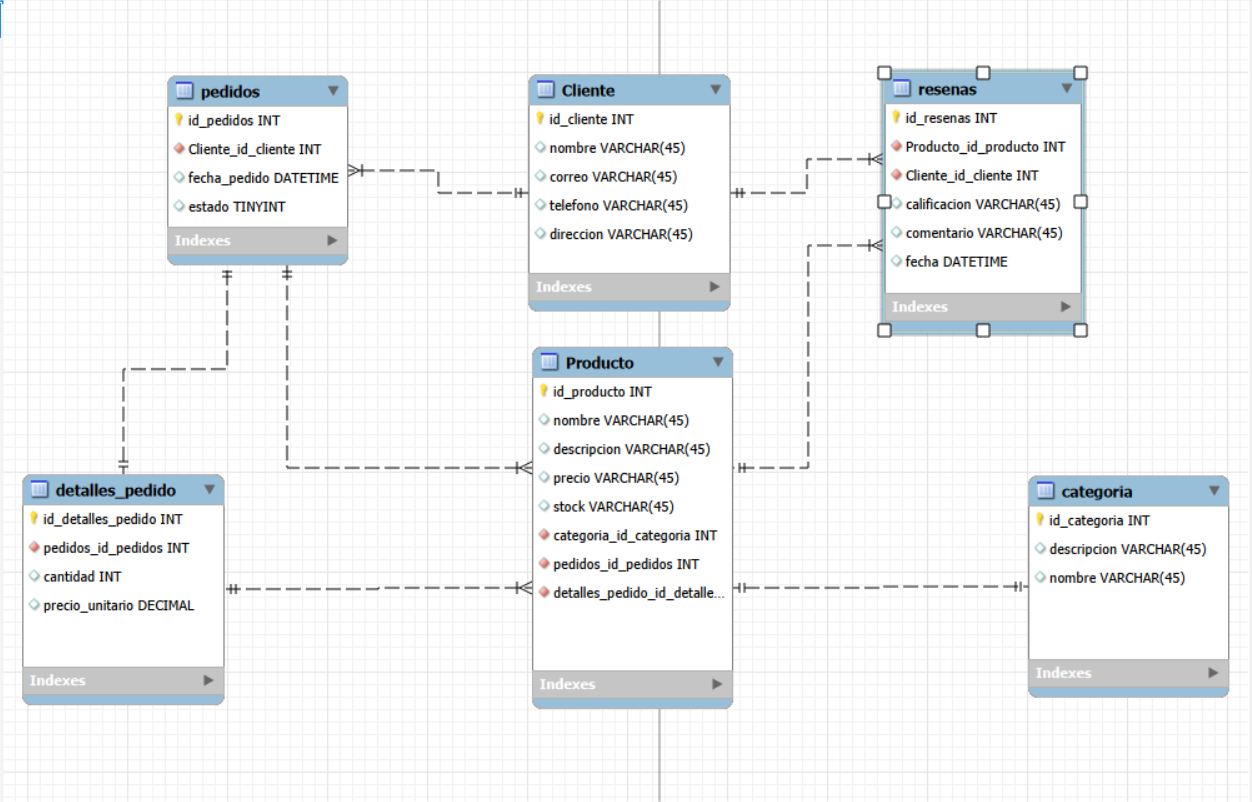
\includegraphics[width=0.8\textwidth]{f1_diagrama_ER.png}
    \caption{Diagrama entidad-relación del Sistema de tienda online}
    \label{fig:diagrama}
\end{figure}

\subsection{Justificación de la normalización}
Al analizar el diagrama Entidad-Relación diseñado, logré identificar que cumple con las formas normales basándonos en las reglas:

\begin{enumerate}
    \item \textbf{Primera Forma Normal (1NF):} El diagrama muestra que todos los atributos de cada entidad son atómicos, o sea que no tiene atributos multivaluados, por ejemplo, en lugar de guardar una lista de productos dentro de un mismo pedido, se creó la tabla \texttt{detalles\_pedido}. Cada entidad está diseñada para almacenar un único valor por campo, cumpliendo la 1NF.
    \item \textbf{Segunda Forma Normal (2NF):} El modelo cumple con la 2NF porque además de cumplir el requisito de satisfacer la 1FN, no tiene dependencias parciales. En las entidades que funcionan como puente (como \texttt{detalles\_pedido}), los atributos dependen de la llave completa que identifica a ese detalle, y no solo de una parte de ella.
    \item \textbf{Tercera Forma Normal (3NF):} Cumple con la 3NF ya que no existen dependencias transitivas; al observar las entidades, nos damos cuenta de que todos los atributos dependen solo de su llave principal, ningún atributo no clave depende de otro atributo no clave, en la tabla \texttt{productos} no ponemos el nombre de la categoría, solo su llave foránea.
    \item \textbf{Cuarta Forma Normal (4NF):} Cumple con la 4NF porque no tenemos ninguna tabla que intente almacenar listas de datos independientes al mismo tiempo, quiere decir que no mezclamos cosas que no tienen nada que ver entre sí en un mismo lugar, separamos los pedidos de las reseñas para evitar que se generen combinaciones de datos sin sentido.
    \item \textbf{Quinta Forma Normal (5NF):} Cumple con la 5NF porque las relaciones entre nuestras entidades son directas, paso a paso y de dos en dos (por ejemplo: el Cliente se relaciona con su Pedido, y el Pedido con el Producto a través del detalle), no tenemos relaciones donde 3 entidades distintas dependan estrictamente unas de otras al mismo tiempo.
\end{enumerate}


\section{Implementación de la base de datos}
A continuación, se presentan los scripts para la creación de las tablas, la optimización con índices y el código de la inserción de datos de prueba.

\begin{lstlisting}[language=SQL, frame=single, caption={Script de creación de esquema, restricciones e índices}]

CREATE DATABASE IF NOT EXISTS tienda_electronica;
USE tienda_electronica;

-- Categorias
CREATE TABLE categorias (
    id_categoria INT AUTO_INCREMENT PRIMARY KEY,
    nombre VARCHAR(100) NOT NULL UNIQUE, -- Nombre único
    descripcion TEXT
);

-- Clientes
CREATE TABLE clientes (
    id_cliente INT AUTO_INCREMENT PRIMARY KEY,
    nombre VARCHAR(150) NOT NULL,
    correo VARCHAR(150) NOT NULL UNIQUE, -- Correo único
    telefono VARCHAR(20),
    direccion VARCHAR(255)
);

-- Productos
CREATE TABLE productos (
    id_producto INT AUTO_INCREMENT PRIMARY KEY,
    nombre VARCHAR(150) NOT NULL,
    descripcion TEXT,
    precio DECIMAL(10,2) NOT NULL,
    stock INT NOT NULL CHECK (stock >= 0), -- Stock no negativo
    id_categoria INT,
    FOREIGN KEY (id_categoria) REFERENCES categorias(id_categoria)
);

-- Pedidos
CREATE TABLE pedidos (
    id_pedido INT AUTO_INCREMENT PRIMARY KEY,
    fecha_pedido DATE NOT NULL,
    estado ENUM('pendiente', 'enviado', 'entregado') DEFAULT 'pendiente',
    id_cliente INT,
    FOREIGN KEY (id_cliente) REFERENCES clientes(id_cliente)
);

-- Detalles_pedido
CREATE TABLE detalles_pedido (
    id_detalle INT AUTO_INCREMENT PRIMARY KEY,
    id_pedido INT,
    id_producto INT,
    cantidad INT NOT NULL CHECK (cantidad > 0),
    precio_unitario DECIMAL(10,2) NOT NULL,
    FOREIGN KEY (id_pedido) REFERENCES pedidos(id_pedido),
    FOREIGN KEY (id_producto) REFERENCES productos(id_producto)
);

-- Resenas
CREATE TABLE resenas (
    id_resena INT AUTO_INCREMENT PRIMARY KEY,
    calificacion INT NOT NULL CHECK (calificacion BETWEEN 1 AND 5),
    comentario TEXT,
    fecha DATE NOT NULL,
    id_producto INT,
    id_cliente INT,
    FOREIGN KEY (id_producto) REFERENCES productos(id_producto),
    FOREIGN KEY (id_cliente) REFERENCES clientes(id_cliente)
);

-- Optimizar la búsqueda de productos por nombre
CREATE INDEX idx_producto_nombre ON productos(nombre);

-- Optimizar la búsqueda de productos por su categoría
CREATE INDEX idx_producto_categoria ON productos(id_categoria);

-- Optimizar la búsqueda del historial de pedidos de un cliente específico
CREATE INDEX idx_pedido_cliente ON pedidos(id_cliente);
\end{lstlisting}

\begin{lstlisting}[language=SQL, frame=single, caption={Script de inserción de datos de prueba}]
USE tienda_electronica;

-- Categorías (3)
INSERT INTO categorias (nombre, descripcion) VALUES
('Teléfonos', 'Smartphones y accesorios celulares'),
('Laptops', 'Computadoras portátiles para uso personal y profesional'),
('Accesorios', 'Cables, audífonos, fundas y periféricos');

-- Clientes (15)
INSERT INTO clientes (nombre, correo, telefono, direccion) VALUES
('Pablo Hernandez', 'pablo@email.com', '5551234', 'Calle 1'),
('Jhovanny Pérez', 'jhovanny@email.com', '5551235', 'Calle 2'),
('Zury Bautista', 'zury@email.com', '5551236', 'Calle 3'),
('Juan Ruiz', 'juan@email.com', '5551237', 'Calle 4'),
('Angel Duenas', 'angel@email.com', '5551238', 'Calle 5'),
('Hugo Soto', 'hugo@email.com', '5551239', 'Calle 6'),
('Sara Rivera', 'sara@email.com', '5551240', 'Calle 7'),
('Paco Luna', 'paco@email.com', '5551241', 'Calle 8'),
('Cecilia Hernández', 'cecilia@email.com', '5551242', 'Calle 9'),
('Raúl Mora', 'raul@email.com', '5551243', 'Calle 10'),
('Nolan Rivera', 'nolan@email.com', '5551244', 'Calle 11'),
('Omar Navarrete', 'omar@email.com', '5551245', 'Calle 12'),
('Lupita Gonzalez', 'lupita@email.com', '5551246', 'Calle 13'),
('José Ruz', 'jose@email.com', '5551247', 'Calle 14'),
('Rogelio Navarrete', 'rogelio@email.com', '5551248', 'Calle 15');

-- Productos (30)(10 teléfonos, 10 laptops, 10 accesorios)
INSERT INTO productos (nombre, descripcion, precio, stock, id_categoria) VALUES
('iPhone 13', 'Teléfono Apple', 15000, 20, 1), ('Galaxy S21', 'Teléfono Samsung', 12000, 15, 1),
('Pixel 6', 'Teléfono Google', 10000, 10, 1), ('Xiaomi Mi 11', 'Teléfono Xiaomi', 8000, 25, 1),
('Moto G100', 'Teléfono Motorola', 7500, 30, 1), ('OnePlus 9', 'Teléfono OnePlus', 11000, 5, 1),
('iPhone 14', 'Teléfono Apple', 18000, 10, 1), ('Galaxy S22', 'Teléfono Samsung', 14000, 12, 1),
('Poco X3', 'Teléfono Poco', 5000, 40, 1), ('Huawei P40', 'Teléfono Huawei', 9000, 8, 1),
('MacBook Air', 'Laptop Apple', 20000, 10, 2), ('Dell XPS 13', 'Laptop Dell', 25000, 5, 2),
('ThinkPad X1', 'Laptop Lenovo', 22000, 7, 2), ('HP Envy', 'Laptop HP', 18000, 12, 2),
('Asus ZenBook', 'Laptop Asus', 17000, 9, 2), ('Acer Swift', 'Laptop Acer', 15000, 15, 2),
('MacBook Pro', 'Laptop Apple', 30000, 3, 2), ('Razer Blade', 'Laptop Razer', 35000, 2, 2),
('MSI Stealth', 'Laptop MSI', 28000, 4, 2), ('Lenovo Legion', 'Laptop Gaming Lenovo', 24000, 6, 2),
('AirPods Pro', 'Audífonos Apple', 5000, 50, 3), ('Galaxy Buds', 'Audífonos Samsung', 3000, 40, 3),
('Sony WH-1000XM4', 'Audífonos Sony', 6000, 15, 3), ('Cable USB-C', 'Cable 2 metros', 200, 100, 3),
('Cargador Rápido', 'Cargador 20W', 400, 80, 3), ('Funda iPhone 13', 'Funda silicona', 300, 60, 3),
('Mica de Cristal', 'Protector de pantalla', 150, 120, 3), ('PowerBank 10000mAh', 'Batería externa', 800, 30, 3),
('Mouse Inalámbrico', 'Mouse Bluetooth', 500, 45, 3), ('Teclado Mecánico', 'Teclado USB', 1200, 20, 3);

-- Pedidos (20)
INSERT INTO pedidos (fecha_pedido, estado, id_cliente) VALUES
('2023-10-01', 'entregado', 1), ('2023-10-02', 'entregado', 2), ('2023-10-03', 'entregado', 3),
('2023-10-04', 'enviado', 4), ('2023-10-05', 'pendiente', 5), ('2023-10-06', 'entregado', 6),
('2023-10-07', 'enviado', 7), ('2023-10-08', 'pendiente', 8), ('2023-10-09', 'entregado', 9),
('2023-10-10', 'enviado', 10), ('2023-10-11', 'pendiente', 11), ('2023-10-12', 'entregado', 12),
('2023-10-13', 'enviado', 13), ('2023-10-14', 'pendiente', 14), ('2023-10-15', 'entregado', 15),
('2023-10-16', 'enviado', 1), ('2023-10-17', 'pendiente', 2), ('2023-10-18', 'entregado', 3),
('2023-10-19', 'enviado', 4), ('2023-10-20', 'pendiente', 5);

-- Detalles de Pedido (25)
INSERT INTO detalles_pedido (id_pedido, id_producto, cantidad, precio_unitario) VALUES
(1, 1, 1, 15000), (1, 21, 1, 5000), (2, 11, 1, 20000), (3, 2, 1, 12000), (3, 22, 1, 3000),
(4, 12, 1, 25000), (5, 3, 2, 10000), (6, 23, 1, 6000), (7, 13, 1, 22000), (8, 4, 1, 8000),
(9, 24, 3, 200), (10, 14, 1, 18000), (11, 5, 1, 7500), (12, 25, 2, 400), (13, 15, 1, 17000),
(14, 6, 1, 11000), (15, 26, 1, 300), (16, 16, 1, 15000), (17, 7, 1, 18000), (18, 27, 2, 150),
(19, 17, 1, 30000), (20, 8, 1, 14000), (20, 28, 1, 800), (15, 29, 1, 500), (1, 30, 1, 1200);

-- Reseñas (10)


INSERT INTO resenas (calificacion, comentario, fecha, id_producto, id_cliente) VALUES
(5, 'Excelente teléfono, muy rápido.', '2023-10-10', 1, 1),
(4, 'Buena laptop, pero la batería dura poco.', '2023-10-11', 11, 2),
(5, 'Me encantó la cámara del S21.', '2023-10-12', 2, 3),
(3, 'Los audífonos están bien, un poco caros.', '2023-10-13', 21, 1),
(5, 'Muy potente para programar.', '2023-10-14', 12, 4),
(4, 'Buen diseño de audífonos.', '2023-10-15', 22, 3),
(5, 'Carga súper rápido.', '2023-10-16', 25, 12),
(2, 'La funda se rayó muy rápido.', '2023-10-17', 26, 15),
(5, 'El mejor mouse que he tenido.', '2023-10-18', 29, 15),
(4, 'Buen teclado, aunque algo ruidoso.', '2023-10-19', 30, 1);

\end{lstlisting}

\section{Consultas y procedimientos almacenados}
Para manipular los datos y aplicar las reglas de negocio, se diseñaron consultas y procedimientos almacenados para no depender de la aplicación externa.

\subsection{Consultas SQL}
Se desarrollaron \texttt{SELECT} con \texttt{JOIN} y funciones de agregación (\texttt{COUNT}, \texttt{AVG}).

\begin{lstlisting}[language=SQL, frame=single, caption={Consulta 1: Listar productos disponibles por categoría, ordenados por precio.}]
SELECT p.nombre AS producto, c.nombre AS categoria, p.precio, p.stock
FROM productos p
JOIN categorias c ON p.id_categoria = c.id_categoria
WHERE p.stock > 0
ORDER BY p.precio ASC;
\end{lstlisting}


\begin{lstlisting}[language=SQL, frame=single, caption={Consulta 2: Mostrar clientes con pedidos pendientes y total de compras.}]
SELECT c.nombre AS cliente, c.correo, COUNT(pe.id_pedido) AS total_pedidos_pendientes
FROM clientes c
JOIN pedidos pe ON c.id_cliente = pe.id_cliente
WHERE pe.estado = 'pendiente'
GROUP BY c.id_cliente;
\end{lstlisting}

\begin{lstlisting}[language=SQL, frame=single, caption={Consulta 3: Reporte de los 5 productos con mejor calificación promedio en reseñas.}]
SELECT p.nombre AS producto, AVG(r.calificacion) AS promedio_calificacion
FROM productos p
JOIN resenas r ON p.id_producto = r.id_producto
GROUP BY p.id_producto
ORDER BY promedio_calificacion DESC
LIMIT 5;
\end{lstlisting}



\subsection{Procedimientos Almacenados (Store Procedures)}
Los procedimientos nos permiten validar condiciones usando \texttt{IF} y frenar transacciones inválidas con \texttt{SIGNAL}.

\begin{lstlisting}[language=SQL, frame=single, caption={Store Procedures para automatizar reglas de negocio y mantener integridad de datos}]
-- Procedimientos almacenados

-- Cambiamos el delimitador a dos diagonales para que mysql entienda que todo el procedimiento es un solo bloque de codigo y no se detenga cuando encuentre los puntos y comas internos
DELIMITER //

-- 1. Registrar un nuevo pedido, verificando el límite de 5 pedidos pendientes y stock suficiente.
-- este procedimiento sirve para automatizar las compras porque primero declaramos variables locales para guardar de forma temporal los datos que vamos a consultar de las tablas, luego usamos SELECT COUNT y SELECT STOCK INTO para meter los resultados dentro de nuestras variables y poder hacer las validaciones del negocio con un IF, si el cliente ya debe 5 pedidos o si no hay stock, usamos signal SQLSTATE '45000' para detener todo por completo y lanzar un error personalizado, evitando que la base de datos se rompa o registre datos falsos;  si todo esta bien, se inserta el pedido y usamos LAST_INSERT_ID para agarrar el id que se acaba de generar en automatico y meterlo directo en detalles_pedido
CREATE PROCEDURE sp_registrar_pedido(
    IN p_id_cliente INT,
    IN p_id_producto INT,
    IN p_cantidad INT,
    IN p_precio DECIMAL(10,2)
)
BEGIN
    DECLARE v_pendientes INT;
    DECLARE v_stock INT;
    DECLARE v_nuevo_id_pedido INT;

    -- contamos cuantos pedidos pendientes tiene este cliente y lo guardamos en la variable
    SELECT COUNT(*) INTO v_pendientes FROM pedidos WHERE id_cliente = p_id_cliente AND estado = 'pendiente';

    -- revisamos cuanto stock tiene el producto actual y lo guardamos en la variable
    SELECT stock INTO v_stock FROM productos WHERE id_producto = p_id_producto;

    IF v_pendientes >= 5 THEN
        SIGNAL SQLSTATE '45000' SET MESSAGE_TEXT = 'Error: El cliente ya tiene 5 pedidos pendientes máximos.';
    ELSEIF v_stock < p_cantidad THEN
        SIGNAL SQLSTATE '45000' SET MESSAGE_TEXT = 'Error: No hay suficiente stock para este producto.';
    ELSE
        -- si pasa los filtros guardamos el pedido usando CURDATE para poner la fecha del dia de hoy en automatico
        INSERT INTO pedidos (fecha_pedido, estado, id_cliente) VALUES (CURDATE(), 'pendiente', p_id_cliente);

        -- guardamos el id generado para no perder la relacion con su detalle
        SET v_nuevo_id_pedido = LAST_INSERT_ID();

        -- insertamos el producto en la tabla puente de detalles_pedido
        INSERT INTO detalles_pedido (id_pedido, id_producto, cantidad, precio_unitario) VALUES (v_nuevo_id_pedido, p_id_producto, p_cantidad, p_precio);
    END IF;
END //


-- 2. Registrar una reseña, verificando que el cliente haya comprado el producto.
-- este procedimiento protege la integridad de las opiniones de la tienda, hacemos un SELECT COUNT cruzando detalles_pedido y pedidos con un JOIN para verificar si existe al menos un registro donde este cliente haya pagado por este producto, si el conteo da cero significa que nunca lo compro, por lo que usamos SIGNAL SQLSTATE para arrojar un error y bloquear la insercion de la resena
CREATE PROCEDURE sp_registrar_resena(
    IN p_calificacion INT,
    IN p_comentario TEXT,
    IN p_id_producto INT,
    IN p_id_cliente INT
)
BEGIN
    DECLARE v_compro INT;

    -- buscamos si hay registros que demuestren que el cliente si compro el producto
    SELECT COUNT(*) INTO v_compro
    FROM detalles_pedido dp
    JOIN pedidos p ON dp.id_pedido = p.id_pedido
    WHERE p.id_cliente = p_id_cliente AND dp.id_producto = p_id_producto;

    IF v_compro = 0 THEN
        SIGNAL SQLSTATE '45000' SET MESSAGE_TEXT = 'Error: Solo puedes hacer reseñas de productos que hayas comprado.';
    ELSE
        INSERT INTO resenas (calificacion, comentario, fecha, id_producto, id_cliente)
        VALUES (p_calificacion, p_comentario, CURDATE(), p_id_producto, p_id_cliente);
    END IF;
END //


-- 3. Actualizar el stock de un producto después de un pedido
-- este procedimiento sirve para manteer actualizado el inventario, lo que hacemos es un UPDATE directo a la tabla de productos usando su llave primaria y le restamos al stock original la cantidad exacta de piezas que el cliente se va a llevar en su compra
CREATE PROCEDURE sp_actualizar_stock(
    IN p_id_producto INT,
    IN p_cantidad_comprada INT
)
BEGIN
    UPDATE productos
    SET stock = stock - p_cantidad_comprada
    WHERE id_producto = p_id_producto;
END //


-- 4. Cambiar el estado de un pedido (ej. de pendiente a enviado)
-- sirve para la logica de logistica de la tienda, usamos un update para modificar el texto del estado de la orden (pendiente, enviado, entregado) guiandonos  por el id_pedido para no alterar las compras de otros clientes
CREATE PROCEDURE sp_cambiar_estado_pedido(
    IN p_id_pedido INT,
    IN p_nuevo_estado VARCHAR(20)
)
BEGIN
    UPDATE pedidos
    SET estado = p_nuevo_estado
    WHERE id_pedido = p_id_pedido;
END //


-- 5. Eliminar reseña de un producto específico, actualizando el promedio de calificaciones
-- aqui primero buscamos cual es el id del producto al que pertenece la resena que queremos borrar y lo respaldamos en una variable local, ya que si la borramos primero perderiamos ese dato; despues de aplicar el delete, hacemos un select combinado con AVG para mostrarle de inmediato al administrador como se recalculo el promedio general de estrellas de ese producto de manera automatica
CREATE PROCEDURE sp_eliminar_resena(
    IN p_id_resena INT
)
BEGIN
    DECLARE v_id_producto INT;

    -- respaldamos el id del producto en nuestra variable antes de borrar el registro
    SELECT id_producto INTO v_id_producto FROM resenas WHERE id_resena = p_id_resena;

    -- borramos la resena de la tabla
    DELETE FROM resenas WHERE id_resena = p_id_resena;

    -- calculamos y mostramos el nuevo promedio real en pantalla
    SELECT p.nombre, AVG(r.calificacion) AS nuevo_promedio
    FROM productos p
    LEFT JOIN resenas r ON p.id_producto = r.id_producto
    WHERE p.id_producto = v_id_producto
    GROUP BY p.id_producto;
END //


-- 6. Agregar un nuevo producto, verificando que no exista un duplicado (mismo nombre y categoría).
-- para evitar errores de captura donde metan dos veces la misma laptop o celular, hacemos un select count buscando si ya hay un registro con exactamente el mismo nombre dentro de la misma categoria, si el sistema encuentra que ya existe, frena la operacion con un signal y le avisa al usuario
CREATE PROCEDURE sp_agregar_producto(
    IN p_nombre VARCHAR(150),
    IN p_descripcion TEXT,
    IN p_precio DECIMAL(10,2),
    IN p_stock INT,
    IN p_id_categoria INT
)
BEGIN
    DECLARE v_existe INT;

    SELECT COUNT(*) INTO v_existe FROM productos
    WHERE nombre = p_nombre AND id_categoria = p_id_categoria;

    IF v_existe > 0 THEN
        SIGNAL SQLSTATE '45000' SET MESSAGE_TEXT = 'Error: Ya existe un producto con ese nombre en esta categoría.';
    ELSE
        INSERT INTO productos (nombre, descripcion, precio, stock, id_categoria)
        VALUES (p_nombre, p_descripcion, p_precio, p_stock, p_id_categoria);
    END IF;
END //


-- 7. Actualizar la información de un cliente (ej. dirección o teléfono)
-- este procedimiento sirve para que el usuario pueda cambiar sus datos de contacto en su perfil, aplicamos un UPDATE directo sobre la tabla clientes y usamos el id_cliente en el WHERE para  que se modifiquen los datos de la persona correcta
CREATE PROCEDURE sp_actualizar_cliente(
    IN p_id_cliente INT,
    IN p_nueva_direccion VARCHAR(255),
    IN p_nuevo_telefono VARCHAR(20)
)
BEGIN
    UPDATE clientes
    SET direccion = p_nueva_direccion, telefono = p_nuevo_telefono
    WHERE id_cliente = p_id_cliente;
END //


-- 8. Generar un reporte de productos con stock bajo (menos de 5 unidades)
-- es una consulta de control para el administrador de la tienda, hace un SELECT filtrando con un WHERE para extraer unicamente los productos que tengan menos de 5 piezas en el inventario, ordenandolos de menor a mayor stock para saber que urge resurtir primero.
CREATE PROCEDURE sp_reporte_stock_bajo()
BEGIN
    SELECT nombre, stock, precio
    FROM productos
    WHERE stock < 5
    ORDER BY stock ASC;
END //

-- regresamos el delimitador al punto y coma que se usa de forma normal en sql
DELIMITER ;
\end{lstlisting}

\end{document}